\section{Simulering af diskrete variable}
Vi vil i følgende afsnit antage, at vi har en stokastisk variabel $U \sim \unif[0,1]$\footnote{Vi vil ikke gå mere i dybden vedrørende simulering af kontinuerte uniforme variable}, som vi vil benytte til at simulere diskrete variable, givet deres pmf.
\begin{thm} \label{thm:simuleringAfDiskreteVaraible}
    Lad $p$ være en pmf over det diskrete udfaldsrum $\{x_1, x_2, \ldots\}$, lad $F_0 = 0$ og
    \begin{equation*}
        F_n = \sum^n_{k = 1} p(x_k), \text{ for } n \in \N.
    \end{equation*}
    Lad $U \sim \unif[0, 1]$, og definer $X = x_n$ hvis $F_{n - 1} < U \leq F_n$, så har $X$ pmf $p$.
\end{thm}

\begin{proof}
    Da $U \sim \unif[0, 1]$ samt $X = x_n$ hvis og kun hvis $F_{n - 1} < U \leq F_n$ er
    \begin{equation*}
        P(X = x_n) = P(F_{n - 1} < U \leq F_n) = F_n - F_{n - 1} = p(x_n)
    \end{equation*}
    fordi $P(F_{n - 1} < U \leq F_n) = P\left(U \leq (F_n - F_{n - 1})\right)$.
\end{proof}

\begin{rem}
Hvis $p$ har tilhørende cdf $F$, så gælder det, at $F_n = F(x_n)$ for $n \geq 1$.
\end{rem}
Følgende algoritme følger af sætning \ref{thm:simuleringAfDiskreteVaraible}, og gør det muligt at simulere diskrete fordelinger, givet den ønskede pmf $p$ og en uniform stokastisk variabel $U$ på intervallet $[0, 1]$.

\begin{algorithm} 
\caption{Simulering af diskrete fordelinger}\label{alg:discreteSimulation} 
\begin{algorithmic}[1] 
\Procedure{Discrete Distrubution} {$p: \{x_1, x_2, \ldots\} \rightarrow [0, 1]$, $U \sim \unif[0, 1]$}
 %$p$ er pmf'en for variablen som ønskes simuleret.
    \State $S := 0$
    \For{$k \in N$}
        \State $S' := S + p(x_k)$ 
        \If{$S < U \leq S'$} \Return $x_k$
        \EndIf
        \State $S := S'$
    \EndFor
\EndProcedure
\end{algorithmic}
\end{algorithm} 



\begin{exmp} \label{exmp:simuleringAfDiskreteVariable}
    Det ønskes at simulere $X \sim \Poi(1)$. Så har $X$ pmf $p(k) = \dfrac{\e^{-1}}{k!}$ for $k \in \N_0$.
    
    Algoritme \ref{alg:discreteSimulation} implementeres i appendix \ref{app:kodeTilSimuleringAfDiskreteVariable}. Her simuleres $n$ stokastiske variable, som følger Poisson fordelingen og måler samtidig frekvensen $F_k$ af hvert udfald i udfaldsrummet $\N_0$.
    Af sætning \ref{thm:law_of_large_numbers} om store tal kan vi approximere $p(k)$ som $\frac{F_k}{n}$ for $k = 0, 1, \ldots$, det benytter vi herefter til at lave følgende plot. 
    \begin{figure}[H]
        \centering
        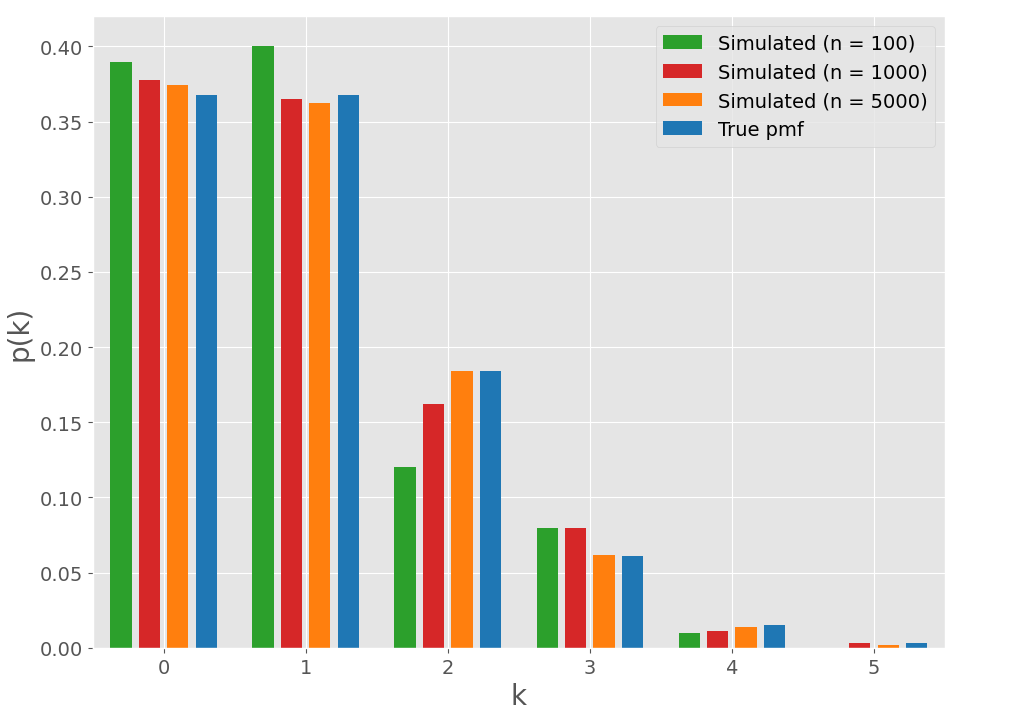
\includegraphics[scale=0.5]{fig/img/poisson.png} 
        \caption{Den simulerede relative frekvens af $k = 0, 1, \ldots, 5$ og den rigtige pmf.}
        \label{fig:simuleringAfPoisson}
    \end{figure}
    Det ses, at den simulerede relative frekvens af $k$ går imod $p(k)$, når $n$ vokser.
\end{exmp}

